\documentclass[11pt]{article}
\usepackage{graphicx}
\usepackage{url}
\usepackage{epigraph}
\usepackage{float}
\usepackage{wrapfig}
\usepackage{listings}
\usepackage{multirow}
\usepackage{hyperref}
\usepackage{amsfonts}
\usepackage{amsmath}
\usepackage{array}
\usepackage{etoolbox}
\usepackage{yax}



\title{\rmfamily\normalfont{Nexus Proof-of-Stake with Tritium Trust}}

\author{Colin Cantrell\\
\and Scott Simon}

\date{October 12, 2018}
    
\begin{document}
\pagenumbering{gobble}

\begin{figure}
    \centering
	
\includegraphics[width=0.44\textwidth]{images/logo.png}
\end{figure}

\maketitle

\newpage
\pagenumbering{arabic}

\bigskip

\section{Introduction}
The Nexus network operates using three channels for producing valid blocks and minting new NXS currency -- two Proof-of-Work channels and one Proof-of-Stake channel. The original Proof-of-Stake channel introduced the concept of trust as a core component to measure consistent and honest contribution by a node to the Nexus network. It followed the philosophy of "everyone has time" in rewarding people for their time investment.\\

\noindent Tritium Trust represents the first in a series of releases implementing the Tritium protocol on the Nexus network. With this release, activated in Nexus version 0.2.5.0, the trust and Proof-of-Stake systems are revised and enhanced. Through these changes, Nexus has laid the groundwork for future releases of the TAO framework to include a Trust and Reputation system as well as Trust Locks integral to the three dimensional chain.\footnote{see "The Nexus Three Dimensional Chain Simplified" by gjsteele71\\ \url{https://steemit.com/bitcoin/@gjsteele71/the-nexus-three-dimensional-chain-simplified}} \\ 

\noindent This paper discusses the details in the Tritium Trust release, specifically with respect to the revised implementation of Nexus Proof-of-Stake.

\bigskip

\section{Definition of Terms}

\subsection{General Terms}

\paragraph{address}- A unique sequence of characters that serves as a public identifier enabling payments to you. When a payment is sent to an address, the blockchain stores that transaction. The resulting \textit{balance} can be thought of as stored "on" that address.

\paragraph{balance}- The amount of a coin that you own. It can represent the total amount, the amount accessed from a single \textit{wallet} (the wallet balance), or the amount accessed by a single \textit{address} (the address balance). All balance is stored on the blockchain, which serves as a ledger recording all transactions. 

\paragraph{coin age}- The blockchain may not store a \textit{balance} in one location. It is often split between multiple locations. Coin age represents an average measure of how long it has been stored in its current locations.  

\paragraph{coinbase transaction}- Proof-of-Work miners add this transaction to each block they mine. It mints (creates) new coins in the form of a reward paid to the address of the miner who created the block.

\paragraph{coinstake transaction}- The Proof-of-Stake counterpart to the coinbase transaction. It mints new coins to pay a reward for creating a new Proof-of-Stake block.

\paragraph{key}- Cryptographic algorithms generally use two keys that form a pair: a private key that is secret to the person holding it, and a public key that can be shared. For cryptocurrencies, the term key typically refers to the private key. This is the key stored in your \textit{wallet}. It can create digital signatures allowing only you to access and spend your coins. The public key is used to derive the public \textit{address}, which is shorter and more easily shared than the key itself.

\paragraph{node}- A computer that is connected to a blockchain network and running the network's blockchain software. This cryptocurrency node stores a copy of the blockchain itself and supports the network by validating and relaying both blocks and transactions. Most cryptocurrency nodes also include a \textit{wallet} interface allowing the computer owner to use the system.

\paragraph{Proof-of-Stake(PoS)}- A form of mining based on ownership of a currency. This ownership represents a "stake" in the sense of an interest in something. PoS miners prove their stake by solving a relatively simple computational problem that requires ownership to perform. By doing so, they become eligible to create a new block and earn a reward. This process is often referred to as "staking your coins", and the resulting reward as the "staking reward".

\paragraph{Proof-of-Work(PoW)}- A form of mining based on a computational problem that is complex to solve but simple to verify. Presenting a solution proves that the work to solve the problem was performed, granting the miner the right to create a new block and earn a reward. 

\paragraph{wallet}- A software program that stores your private \textit{keys} and corresponding \textit{addresses} enabling access to your \textit{balance} on the blockchain. A wallet does not actually store your coins, only your keys. The wallet balance represents the value stored on the blockchain that is accessible by the keys in the wallet.

\subsection{Nexus Terms}

\paragraph{block age}- For Nexus Proof-of-Stake, this refers to the amount of time since a wallet successfully mined its last PoS block and added it to the blockchain. In other words, how old is the most recent PoS block created by that wallet? 

\paragraph{Genesis}- The initial phase of Nexus Proof-of-Stake that allows a new wallet to participate in staking. Each wallet only performs this process once. When a wallet successfully mines its first PoS block, the Genesis process creates a \textit{trust key} in the wallet, which is used for all PoS from that point forward.

\paragraph{Genesis transaction}- The coinstake transaction of the PoS block found by a wallet during its initial Genesis phase.

\paragraph{Trust transaction}- The coinstake transaction of any PoS block found after the wallet completes its Genesis phase. 

\paragraph{trust key}- The private key created in your wallet by the Genesis process. The public NXS address associated with this key is used for all staking reward payments. The staking process also moves the current wallet balance and stores it on this address, along with a record of the \textit{trust score}.

\paragraph{trust score}- Reflects the network’s internal level of trust assigned to a trust key as a measure of the equivalent time the key owner has operated a node in an honest, trustworthy, and timely manner. This measure of time is not absolute. It is accrued during normal operation, but the accrued amount can be reduced when not honest, trustworthy, or timely.

\paragraph{TAO framework}- The three phases for implementing the Nexus three dimensional chain, named Tritium, Amine, and Obsidian respectively. Each represents a major update implementing one dimension of the overall architecture, and may be comprised of one or more releases. 

\paragraph{Tritium}- The first phase of implementing the Nexus three dimensional chain, as defined in the Tritium White Paper\footnote{Nexus: The Tritium Protocol \url{https://nexusearth.com/tritium-white-paper/}}. Tritium itself will be comprised of a series of releases: Tritium Trust, the Nexus Tritium Wallet, and Tritium Core. Tritium Trust implements changes to the trust and PoS system, the Tritium Wallet provides a completely updated wallet experience and implements the interface layer of the architecture, and Tritium Core implements the remaining major architectural updates needed for full implementation of the protocol. \\

\bigskip

\section{Proof-of-Stake}

\subsection{What is Proof-of-Stake?}
The concept of Proof-of-Stake was first introduced in 2012 by King \& Nadal\footnote{King, S.; Nadal, S. (August 12, 2012). ”PPCoin: Peer-to-peer crypto-currency  with  proof-of-stake” \url{https://peercoin.net/assets/paper/peercoin-paper.pdf}} as a proposal to develop a form of mining that addressed the growing issue of energy consumption related to Bitcoin Proof-of-Work mining. It developed the idea of using proof of ownership of a currency as a means for granting the ability to mine blocks on the blockchain. These blocks would include a \textit{coinstake} transaction that rewarded the currency owner in a manner similar to how \textit{coinbase} transactions reward Proof-of-Work miners.\\

\noindent Early incarnations of Proof-of-Stake built around the idea of \textit{coin age}. Upon reaching a specified coin age, the currency owner would gain the ability to stake a new block on the blockchain.\\

\noindent This design elegantly solved the issue of energy efficiency, but had the drawback that, unlike other forms of mining, the currency owner didn't have to do anything. They could simply leave their wallet off, and only activate it upon reaching the age level needed to earn rewards without contributing to the network as a whole.\\

\noindent As a result, Proof-of-Stake was gradually refined. It remained a form of energy efficient mining, but evolved into a mechanism whereby currency holders can earn rewards proportional to the size of their holdings in return for keeping a node up and running at all (or nearly all) times, thus contributing to the operation and security of the blockchain network.\\

\subsection{Staking Concepts}

\paragraph{Time} ~\\
Proof-of-Stake introduced time as an input to mining, initially through the use of coin age. Using time in this manner inhibits the application of raw computational power to solve blocks more quickly, thus promoting energy efficiency. Requiring a significant time investment to stake successfully also introduces an external cost to any potential attacker. This improves network security. 

\paragraph{Weight} ~\\
Different Proof-of-Stake systems use varying ideas for the concept of weight. Basically, all of these introduce an approach where the ability of currency owners is weighted in such a manner that some have a higher chance to generate blocks than others. Coin age based systems were often weighted based on the number of coins owned, so if two people had the same holding period, but one had twice as many coins as the other, that one would have twice as much opportunity to mine staking blocks.

\paragraph{Minting Rate} ~\\
This rate, expressed as an annual percentage, is used to calculate the size of the coinstake reward in a PoS block from the time invested in creating it and the overall PoS balance. \\

\noindent As PoS grew more popular, minting rate became more commonly referred to as \textit{interest rate} because it operates in a similar manner and people already have an understanding of that term. However, anyone staking should understand that their coins are \textbf{not earning interest}. They are \textbf{mining staking rewards} in return for helping operate and secure the blockchain network.

\paragraph{Distribution Problem} ~\\
A pure PoS-based currency suffers from a chicken-and-egg problem that you cannot mine staking blocks without coins to stake. Those coins must first be minted by another process. Therefore, most currencies that use Proof-of-Stake also employ an initial distribution based on Proof-of-Work mining, at least temporarily.\\

\noindent Although Nexus uses 3 mining channels primarily to enhance security, this design also supports initial distribution via the Proof-of-Work channels.

\paragraph{Nothing At Stake Problem} ~\\
Proof-of-Work mining requires the consumption of large amounts of energy, which is a valuable resource. A basic Proof-of-Stake system, on the other hand, only uses resources already within the network, and you don’t lose anything for behaving dishonestly or signing all blocks on any fork in the chain, then attempting to build on all forks. There is no cost or “nothing at stake” for doing so. It is a hypothetical problem that nevertheless must be addressed by any staking system.\\

\noindent In addition to other benefits, the use of multiple channels in Nexus also addresses this problem, as the disparate channels keep each other honest. The Nexus network also uses the concept of trust to create a cost to misbehavior. 

\paragraph{51\% Attack} ~\\
As with other forms of mining, Proof-of-Stake systems can potentially be exposed to a 51\% attack that gives the attacker control of the network. Under this type of system, however, it requires an attacker to gain control of at least 51\% of the currency on the network. This becomes incredibly expensive to do, and thus highly unlikely, especially when you add limitations to block frequency and combine it with a significant time requirement for generating staking weight.\\

\noindent Within Nexus, not only is it highly unlikely a 51\% attack could occur on the Proof-of-Stake channel, but an attacker would also have to gain control of both Proof-of-Work channels to be successful. \\

\paragraph{Inflation} ~\\
Defining the minting rate is an important aspect of any staking system. Too low and rewards are not significant enough to encourage nodes to stake. Too high and the resulting inflation of the currency supply will erode its value, especially when compounded over time. Inflation can rapidly become the nemesis for systems promising excessively high rewards. \\

\noindent The Nexus initial distribution will create a supply of 78 million NXS, ending on September 23, 2024. After that, it will follow an inflationary model based on the annual inflation of gold supply from mining. Gold has kept its value for centuries, so this level of inflation has proven economically sustainable. \\

\noindent Under this model, after the initial distribution ends each Proof-of-Work channel will inflate supply by 1\% per year, and the Proof-of-Stake channel will allow a maximum of 3\%. This 3\% value could only be realized if the entire NXS supply were staked at the maximum Interest Rate. Realistically, Proof-of-Stake inflation will likely fall in line with the other two minting channels.\\

\bigskip

\section{Nexus Proof-of-Stake}
The Tritium Trust release builds on the previous Nexus Proof-of-Stake system. It employs many of the staking concepts developed in previous staking systems, enhances them, and adds new concepts that further enhance performance and security for Proof-of-Stake.\\

\subsection{Genesis}
Before a new wallet can stake successfully on the Nexus network, it must first create a trust key. This key is created by successfully mining its first Proof-of-Stake block, a process referred to as Genesis. \\

\begin{figure}[h!]
    \centering
    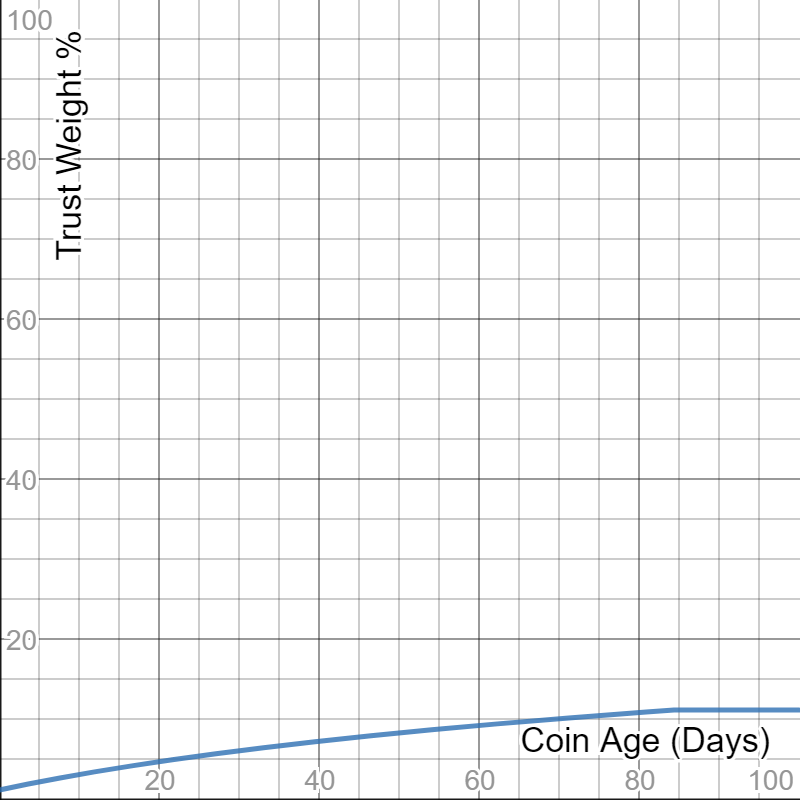
\includegraphics[width=0.63\textwidth]{images/preGenesisTrustWeight.png}
    \caption{Trust Weight pre-Genesis \label{fig:preGenesisTrust}}
\end{figure}

\noindent While staking for Genesis, the node will slowly build Trust Weight (see section 4.2). Over time, this added weight increases the chances of mining a PoS block and generating a Genesis transaction. The pre-Genesis value for Trust Weight only applies to the Genesis process and is based on coin age. It caps at a level of 11\% of maximum, as shown in Figure \ref{fig:preGenesisTrust}.\\

\noindent As part of the Genesis transaction, the wallet also creates the trust key and transfers all balance to that key's address for staking. This has no impact on the wallet balance, besides moving it to the new address.\\

\noindent Under Tritium Trust, each wallet will only perform Genesis once. After it creates a trust key, it will continue to use it for the remainder of the lifetime of that wallet.\\


\subsection{Trust}
Upon creating a new trust key, the network immediately begins to build the internal trust score associated with that key. Continued staking will generate additional Trust transactions whenever the node successfully mines a Proof-of-Stake block. Each additional transaction rewards the wallet owner for continuing to operate their node.\\

\noindent Continued staking also sustains the trust score and allows it to keep accruing. As long as the trust key does not undergo Decay (see section 4.5) or get penalized for misbehavior, trust score will continue to grow.\\

\begin{figure}[h!]
    \centering
    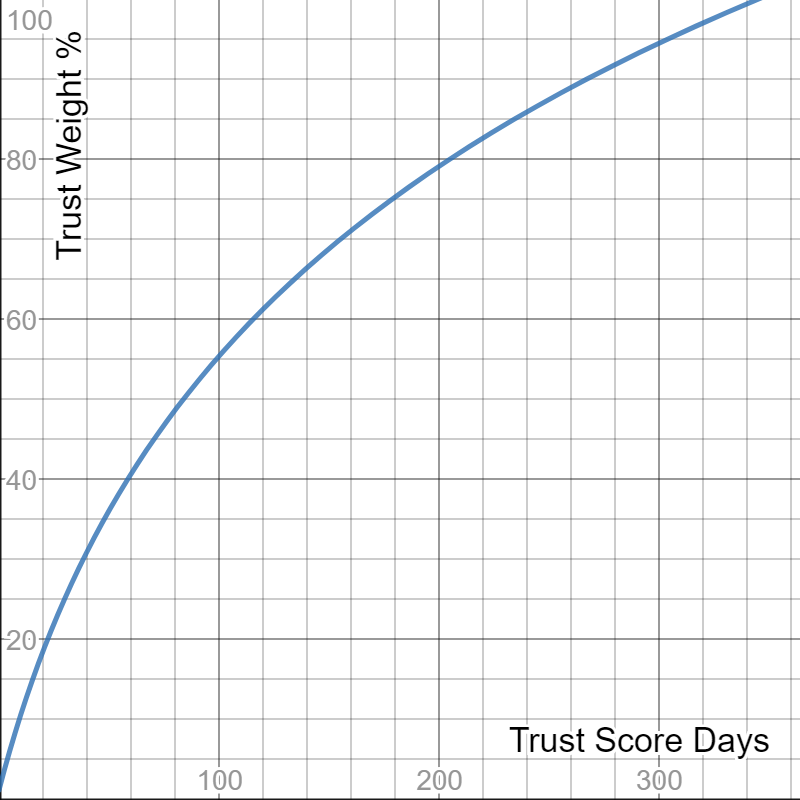
\includegraphics[width=0.63\textwidth]{images/trustWeight.png}
    \caption{Trust Weight \label{fig:trustWeight}}
\end{figure}

\noindent The internal trust score is important for Nexus Proof-of-Stake, because it indicates the network's level of trust in the associated trust key. With more trust, the network awards that key a higher weight for staking and a higher Interest Rate (see Section 4.3). The weight it awards is indicated by the Trust Weight. A higher value for Trust Weight increases the chances of successfully mining PoS blocks.\\

\noindent Figure \ref{fig:trustWeight} depicts the relationship between trust score and Trust Weight. It shows how Trust Weight, expressed as a percentage of its maximum possible value, grows as accrued trust score, expressed as days of time, increases.\\

\noindent As with the Genesis transaction, Trust transactions will also transfer any new NXS sent to the wallet onto the trust key's address for staking. \\

\subsection{Interest Rate (Minting Rate of Staking Rewards)}
Unlike Proof-of Work mining, Nexus Proof-of-Stake does not have a set reward for finding blocks. Instead, the reward size is calculated from the trust key's current Interest Rate (minting rate), the time it took to find the block, and the wallet balance. The Genesis stage uses a fixed rate of 0.5\% (annual). After Genesis, the network determines Interest Rate from its current level of trust, as measured by the accrued trust score.\\

\begin{figure}[h!]
    \centering
    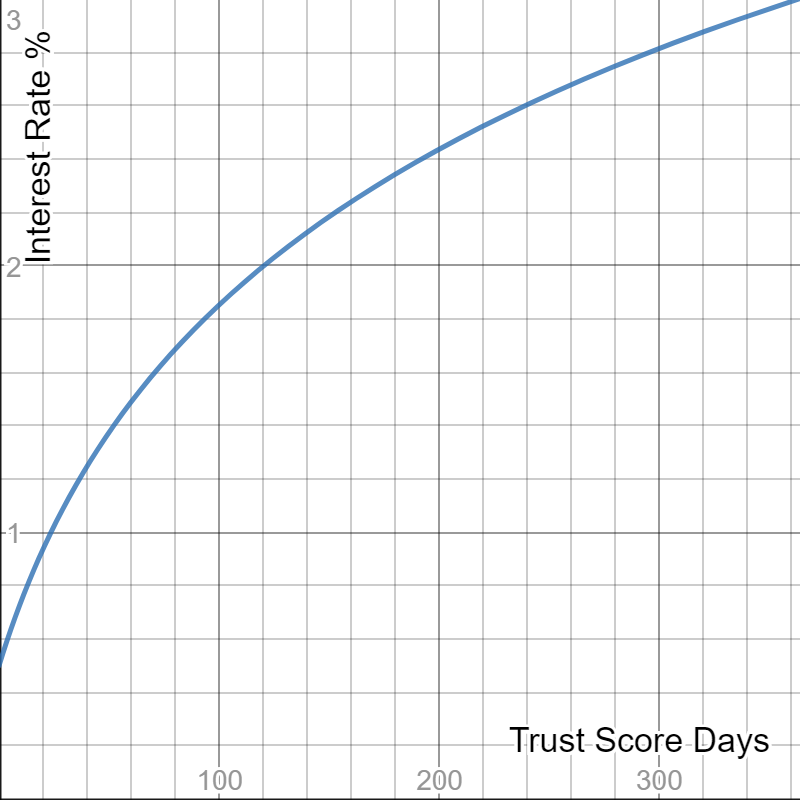
\includegraphics[width=0.63\textwidth]{images/interestRate.png}
    \caption{Interest Rate \label{fig:interestRate}}
\end{figure}

\noindent This annual interest rate ranges from the starting value of 0.5\% to a maximum of 3.0\% after the trust key has attained one year worth of aggregate trust score. \\

\noindent Figure \ref{fig:interestRate} depicts how Interest Rate, expressed as an annual percentage, grows as accrued trust score, expressed in days of time, increases. Interest Rate caps when it reaches the maximum value of 3\%.\\

\subsection{Block Weight}
The Block Weight represents a second weight value. It combines with Trust Weight (see section 4.2) to increase the chances for mining a new PoS block.\\

\noindent Block Weight derives from the amount of time since the wallet last mined a PoS block, as measured by its block age. The older the last block, the more weight it contributes to finding a new one, up to a maximum value reached after three days. \\

\noindent During Genesis, the wallet has not yet mined any Proof-of-Stake blocks. The block age value remains zero, and so does the Block Weight. Upon mining the first PoS block, Nexus begins measuring the age of that block, and Block Weight will begin increasing. \\

\noindent Whenever the wallet mines an additional PoS block, Nexus begins measuring the block age of the new block in place of the prior one. This has the effect of resetting Block Weight and it starts growing again as the new block age increases. \\

\noindent Figure \ref{fig:blockWeight} depicts how Block Weight, expressed as a percentage of maximum value, grows as block age increases.\\

\begin{figure}[h!]
    \centering
    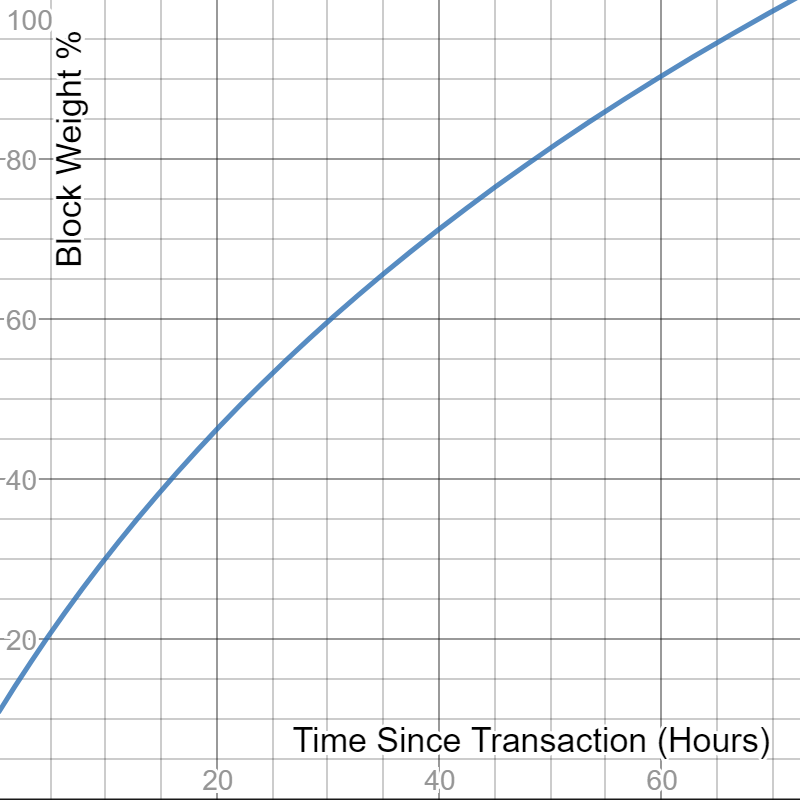
\includegraphics[width=0.63\textwidth]{images/blockWeight.png}
    \caption{Block Weight \label{fig:blockWeight}}
\end{figure}

\noindent If, after 3 days (72 hours), Block Weight reaches 100\%, the trust key will begin to undergo Decay (see section 4.5).\\


\subsection{Decay}
Tritium Trust introduces the process of Decay if a wallet fails to mine blocks in a timely manner. To stay timely, the wallet must mine a new PoS block before the block age of the previous one reaches three days. This time limit is reached when the Block Weight reaches 100\%. \\

\noindent If the wallet reaches the 3-day limit without mining a new PoS block, the trust key does not expire. Instead, the trust score associated with that key will reset back to the level of its previous Trust transaction. Any trust score added since then is lost. Then it begins to decay from that point. Trust score decays at a 3:1 ratio to the rate it was accrued.\\

\begin{equation}
\resizebox{.50\hsize}{!}{$T_s = T_p - 3 \cdot (a_{b} - 259200)$}
\end{equation}

\noindent Where $T_s$ = new trust score, $T_p$ = prior trust score at last transaction, $a_{b}$ = block age (time since last PoS block, in seconds), and 259200 is three days expressed in seconds.\\

\noindent Normally, Trust Weight depicted in Figure \ref{fig:trustWeight} moves forward along the curve as trust score grows. During Decay, it effectively moves backward along the same curve. The same would be true of Interest Rate in Figure \ref{fig:interestRate}. \\

\noindent Decay ends if, at any time, the wallet mines a new stake block and generates a Trust transaction. Trust score begins accruing again from that point. \\

\noindent The benefit of Decay in Tritium Trust is that trust keys no longer expire. They simply add or subtract trust score. Those who have invested a lot of time building trust will not have it expire from a random event such as a power outage. Trust score might decay somewhat, but it can be earned back.\\

\noindent The time investment that it takes to build trust score, combined with this introduction of the ability to both add and subtract trust score, also supports administration of trust penalties for misbehavior or dishonesty, and forms the basis for future application as part of a Trust and Reputation system within the Nexus TAO framework.\\

\subsection{Use of Coin Age in Nexus}
Enough different Proof-of-Stake systems have used coin age in different ways that it can become a matter of confusion. While this document already shows coin age in the places where Nexus uses it, summing this up in one section will clarify it better.\\

\noindent With one exception, Nexus only uses coin age during the Genesis stage. Coin age determines the minimum time to wait before you can stake a new wallet. It also determines Trust Weight and the reward included in the Genesis transaction.\\

\noindent After Genesis mines the first PoS block, Tritium Trust uses trust score and block age in place of coin age. It only considers coin age if you add new NXS to your wallet. In that case, the previous balance stored on the trust key's address earns a reward based on block age, but the new NXS amount only earns a reward for the time after adding it to the wallet (its coin age). The next Trust transaction will take that into account while also moving the new amount onto the trust key's address. After that, the coin age is no longer considered. \\

\noindent Note that, after Genesis, coin age has no impact on trust score, Trust Weight, Block Weight, or Interest Rate.\\

\bigskip

\section{Begin Staking with a New Wallet}

\subsection{Establishing a Trust Key}
Trust is not something easily earned in real life. Nor is it easily established in Nexus Proof-of-Stake. Establishing a new trust key is a process. This process can take a fair amount of time, especially for smaller balances.\\

\noindent After Genesis successfully mines the initial PoS block and creates the trust key, the trust score associated with that key begins accruing but starts small. This results in a low Trust Weight value that does not contribute much weight for mining additional blocks. Trust transactions remain infrequent. \\

\noindent It is normal at this stage if it doesn't mine a new PoS block within the required three day period. As the key is new, Decay immediately reduces trust score to its starting value (the trust level of its prior transaction) when Block Weight reaches 100\%.\\ 

\noindent From that point, Block Weight will stay at 100\% while it continues to search for a PoS block, but Trust Weight and Interest Rate revert to minimum starting values (1.11\% and 0.5\% respectively). These values will not change until it mines a stake block and generates a Trust transaction. Then, trust score begins to grow again.\\

\noindent This cycle may repeat multiple times before a new trust key can generate enough Trust transactions with enough frequency to avoid Decay and accumulate trust score. This is normal. It is all part of earning trust.\\

\subsection{Nexus Staking Requirements}

\paragraph{Minimum Balance} ~\\
No matter how much NXS you have, you can operate a node and mine rewards using Nexus Proof-of-Stake. There is no minimum amount required. You are guaranteed to receive staking rewards calculated using the starting 0.5\% Interest Rate. \\

\noindent However, if you have a higher balance, it will find PoS blocks and create Trust transactions more frequently, and therefore have a greater likelihood of growing trust score to higher levels. This also grows the Interest Rate for calculating staking rewards, up to the maximum of 3\%.

\paragraph{Minimum Coin Age} ~\\
Before a wallet can attempt Genesis and mine its first PoS block, it requires a minimum coin age of 72 hours. A new wallet that just received its first NXS must wait this long to begin staking. Any additional sending or receiving of NXS during this time alters the coin age, which may increase how long it must wait. 

\paragraph{Hardware} ~\\
You can stake NXS on any system supported by the latest Nexus wallet version. Currently, that includes computers running 64-bit versions of Windows, MacOS, or Linux. Devices such as mobile phones or Raspberry Pi are not yet supported. The staking process does not require a high powered machine, though. Many use older laptops or mini-systems like the Intel NUC to minimize power usage. 

\paragraph{Maturity} ~\\
Proof-of-Stake is a form of mining and, as with Proof-of-Work, must wait a minimum period for the staking transaction to mature. For Nexus, maturity takes 120 blocks (around 90 minutes). During this time, the wallet balance will display as "Staking" and not be available for other use. If you send additional NXS to the wallet during the maturity period, it will be available immediately.

\paragraph{Three Day Requirement} ~\\
As previously noted, a wallet must successfully mine a new PoS block and generate a Trust transaction within three days of its prior one. If not, the trust score will experience Decay. \\

\bigskip

\section{Technical Details}
This section specifies the detailed formulae Tritium Trust uses to calculate values discussed in the prior sections. These replace the now-obsolete calculations originally documented in the Nexus white paper.\footnote{Nexus: A Peer-to-Peer Network \url{https://nexusearth.com/nexus-white-paper/}}

\subsection{Trust Weight}
\noindent As previously discussed, Tritium Trust uses two different calculations for Trust Weight, one based on coin age during the Genesis process and one based on current trust score for the remainder of staking.\\

\noindent The internal value of Trust Weight ranges from 1 to 90, although it is commonly expressed as a percentage of its maximum value.\\

\paragraph{Genesis Trust Weight} ~\\
Tritium Trust only uses this while attempting to mine the initial PoS block.

\begin{equation}
\resizebox{.65\hsize}{!}{$W_{t} = Min(10.0, \frac{9.0 \cdot ln(\frac{2 \cdot a_c}{7257600} + 1)}{ln(3)} + 1.0)$}
\end{equation}

\noindent Where $a_c$ is the current coin age.\\

\paragraph{Ongoing Trust Weight} ~\\
After Genesis mines the initial PoS block and creates the trust key, Tritium Trust calculates Trust Weight using this method.
 
\begin{equation}
\resizebox{.65\hsize}{!}{$W_{t} = Min(90.0, \frac{44.0 \cdot ln(\frac{2 \cdot T_{s}}{7257600} + 1)}{ln(3)} + 1.0)$}
\end{equation}

\noindent Where $T_{s}$ is the current trust score.\\


\subsection{Interest Rate (Minting Rate of Staking Rewards)}
\noindent The staking reward included in the Genesis transaction is calculated using the starting rate of 0.5\%. All subsequent rewards for mining PoS blocks use a minting rate calculated from accumulated trust score.\\
 
\begin{equation}
\resizebox{.65\hsize}{!}{$R_{m} = \frac{0.025 \cdot ln(\frac{9 \cdot T_{s}}{31449600} + 1)}{ln(10)} + 0.005$}
\end{equation}

\noindent Where $T_{s}$ is the current trust score and $R_{m}$ is the resulting minting rate (interest rate).\\


\subsection{Staking Rewards}
\paragraph{Genesis Transaction} ~\\
\begin{equation}
\resizebox{.35\hsize}{!}{$S_{r} = \frac{C_{w} \cdot 0.005 \cdot a_c}{31449600}$}
\end{equation}

\noindent Where $C_{w}$ is the current wallet balance and $S_{r}$ is the staking reward.

\paragraph{Trust Transaction} ~\\
The staking reward received in a Trust transaction has two possible components. The first part is the reward for balance stored on the trust key's address, based on the block age (time since last staking transaction). The second part accounts for any new NXS balance added to the wallet. This NXS only earns rewards for the time since adding it.\\

\begin{equation}
\resizebox{.35\hsize}{!}{$S_{t} = \frac{C_{t} \cdot R_{m} \cdot a_{b}}{31449600}$}
\end{equation}

\noindent Where $C_{t}$ is the balance on trust key's address, $a_{b}$ is the block age, and $S_{t}$ is the staking reward from the trust key.\\

\begin{equation}
\resizebox{.35\hsize}{!}{$S_{n} = \frac{C_{n} \cdot R_{m} \cdot a_c}{31449600}$}
\end{equation}

\noindent Where $C_{n}$ is any new NXS added to the wallet, $a_c$ is the coin age of that new balance, and $S_{n}$ is the resulting staking reward. New NXS is then transferred to the trust key's address for further staking.\\

\noindent The total reward for a trust transaction $S_{r} = S_{t} + S_{n}$\\


\subsection{Block Weight}
Tritium Trust only calculates Block Weight after Genesis mines the initial PoS block. It uses the block age of the most recent PoS block mined. \\

\noindent The numeric value of Block Weight ranges from 1 to 10, although it is commonly expressed as a percentage of its maximum value.\\

\begin{equation}
\resizebox{.65\hsize}{!}{$W_{b} = Min(10.0, \frac{9.0 \cdot ln(\frac{2 \cdot a_{b}}{259200} + 1)}{ln(3)} + 1.0)$}
\end{equation}\\


\subsection{Stake Weight}
Stake Weight is a derivative measure that depicts the combined weight effect of Trust Weight and Block Weight on overall chances to generate a block. The Required Threshold (see Section 6.6) uses Trust Weight and Block Weight directly, so the value of Stake Weight is for informative purposes only.

\begin{equation}
\resizebox{.30\hsize}{!}{$W_{s} = W_{t} + W_{b}$}
\end{equation} 

\noindent As shown previously, internal values for Trust Weight range from 1-90 and Block Weight from 1-10. Thus, Stake Weight will range from 2-100, and can be directly expressed as a percentage.\\


\subsection{Required Threshold}

\begin{equation}
\resizebox{.5\hsize}{!}{$R_{t} = \frac{(108 - W_{t} - W_{b}) \cdot 1000}{(C_{w} + S_{r})}$}
\end{equation}


\noindent The value for Energy Efficiency Threshold must be above this value for the wallet to attempt stake block generation.\\


\subsection{Energy Efficiency Threshold}

\begin{equation}
\resizebox{.22\hsize}{!}{$E_{t} = \frac{100 \cdot t_{b}}{N_{once}}$}
\end{equation}

\noindent Where $t_{b}$ is the time since the last block was added to the blockchain, in seconds.\\

\noindent The Tritium Trust staking process will iterate over the process of attempting to find a block hash that meets PoS difficulty requirements, incrementing $N_{once}$ with each iteration. Whenever this causes the value for the Energy Efficiency Threshold to fall below the Required Threshold, it will stop.\\

\noindent As the time since the last block increases, so will the Energy Efficiency Threshold and it can begin iterating again. Higher Trust Weight, Block Weight, and wallet balance reduce the Required Threshold, thus allowing for a greater number of iterations and increasing the possibility of mining a block.\\

\noindent This continues until it finds a PoS block or it receives a new block from the network. If it receives a new block, the process resets and starts over.\\

\noindent Another way of looking at this process is through the understanding of Proof-of-Stake as a form of mining. In effect, the math, weights, and thresholds only exist to determine the effective "hash rate" for Proof-of-Stake. In the end, this hash rate determines how often, on average, it will find a block and earn a reward, just like with Proof-of-Work mining.\\

\noindent If you mine using Proof-of-Work, and wish to generate more results, then you add more hash rate. With Proof-of-Stake, you do the same. The most effective way to increase Proof-of-Stake hashing is to add more balance to the wallet, though building trust also does so. \\

\noindent Through this process, the staking algorithm produces a non-intensive, efficient process\footnote{One with a variable "hash rate" typically a few h/s and not Mh/s} based on the parameters of the wallet’s trust key, avoiding the need for a lot of expensive hardware and energy consumption.\\

\bigskip

\section{Summary}

With the activation of Nexus 0.2.5.0, the Tritium Trust release revises and enhances the Nexus Proof-of-Stake system as a method for mining NXS. It eliminates the expiration of trust keys and implements trust score as both a measure of the network's level of trust and as a primary input for determining updated staking parameters.  \\

\noindent Trust score can both increase through continued mining of PoS blocks in a timely manner, and decrease through the process of Decay. This lays the groundwork for further development of Trust and Reputation within the Nexus architecture as part of the overall TAO framework. \\

\bigskip
\bigskip

\section*{Acknowledgements}

Many thanks to Dino Farinacci for his assistance in editing and structuring this document. His experience in writing technical content helped greatly improve the final result. Also thank you to Anastasiya Maslova and Mike Casey for their suggestions and input.

\end{document}
